\section{高速化の方針}

高速化の方針として逐次プログラミングにおける最適化と並列化の両方を考える.

\section{逐次プログラムにおける高速化手法}

\subsection{データ変更の有無による条件分岐の除去 \label{sss:no_set}}

\figref{src:reg} に示した実装では,reg クラスのインスタンスの値を更新する方法としてブロッキング代入とノン・ブロッキング代入の 2 つが存在する.

ブロッキング代入について考える.reg クラスのインスタンスにブロッキング代入が行われた時に curr\_ の値を書き換える.

一方でノン・ブロッキング代入について考える.
reg クラスのインスタンスにノン・ブロッキング代入が行われた時にメンバ変数 set\_ を true にし,メンバ変数 next\_ に値を代入する.
そして reg::Update 内では set\_ が true の時だけ next\_ をメンバ変数 curr\_ に代入する.
これは reg クラスのインスタンスの値を変更したサイクルのみで,
その reg クラスのインスタンスの値を次サイクルに移る前に新しい値に更新することを意味する.

\figref{src:reg} に示した実装では,
更新されない reg クラスのインスタンスの curr\_ と next\_ の値が同じであるため,代入する処理を行う必要はない.
よって set\_ 変数を用いて不要な代入を避けている.
reg クラスのインスタンスの更新頻度が低い回路であればこの実装が効率的である.

提案手法について述べる.
この set\_ 変数が true の時のみ代入するのではなく,
次サイクルに移る前に next\_ の値を curr\_ に常に代入するようにする.
こうすることによって分岐のオーバーヘッドが無くなるため,ノン・ブロッキング代入が頻繁に行われる回路で速度向上が期待できる.

% SWoPP より追加

\begin{figure}[tb]
 \lstinputlisting[language=c++]{src/reg_no_set.cc}
 \caption{条件分岐を除去した reg クラス}
 \label{src:reg_no_set}
\end{figure}

\figref{src:reg_no_set} に提案手法の実装を示す.
\figref{src:reg} の実装から set\_ 変数を除いている.

% 追加ここまで


\subsection{値を配列として格納しメモリ配置を工夫} \label{sss:mem_copy}

\begin{figure}[t]
 \centering
 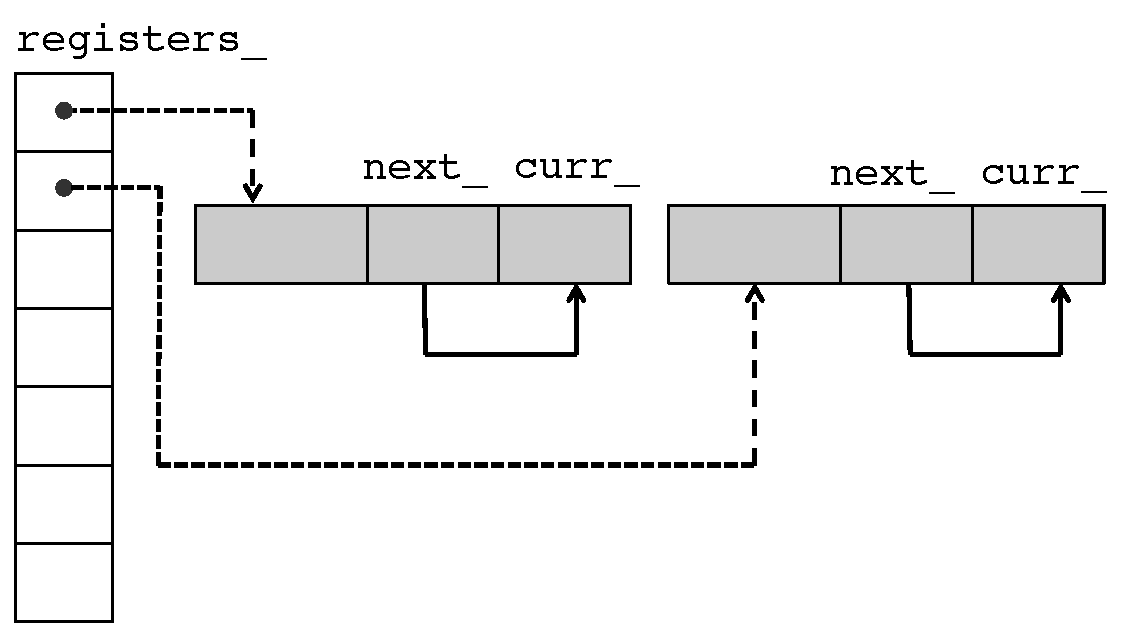
\includegraphics[clip,width=\linewidth-30pt]{registers_orig}
 \caption{ArchHDL における reg クラスのインスタンスの処理の様子}
 \label{fig:regs}
\end{figure}

\figref{fig:regs} は ArchHDL における reg クラスのインスタンスの処理の様子である.
\figref{src:class_singleton} の 44 行から 46 行の処理を表している.
reg クラスのインスタンスが灰色に塗られており,左からクラスのメタデータ,next\_, curr\_ を表している.
左側の大きな枠が\figref{src:class_singleton} の 18 行の \verb`std::vector` 型の registers\_ である.
実線矢印は代入を表し.点線矢印はポインタ参照を表す.

ArchHDL ではノン・ブロッキング代入をシミュレーションするために registers\_ の値を上から順に辿り,
reg クラスの各インスタンスのポインタを取得する.
そして reg クラスの全インスタンスの reg::Update() メソッドを呼ぶ.

\ref{sss:no_set} 節で述べたデータ変更の有無による条件分岐の除去を行うと reg::Update() メソッド内で行なっている
reg クラスのインスタンスの curr\_ に next\_ の値を代入する処理は
毎サイクル全 reg クラスのインスタンスで実行されることになる.

この代入する処理と reg::Update() メソッドの関数呼び出しの 2 つのオーバーヘッドが ArchHDL の高速化を妨げている.

\begin{figure}[t]
 \centering
 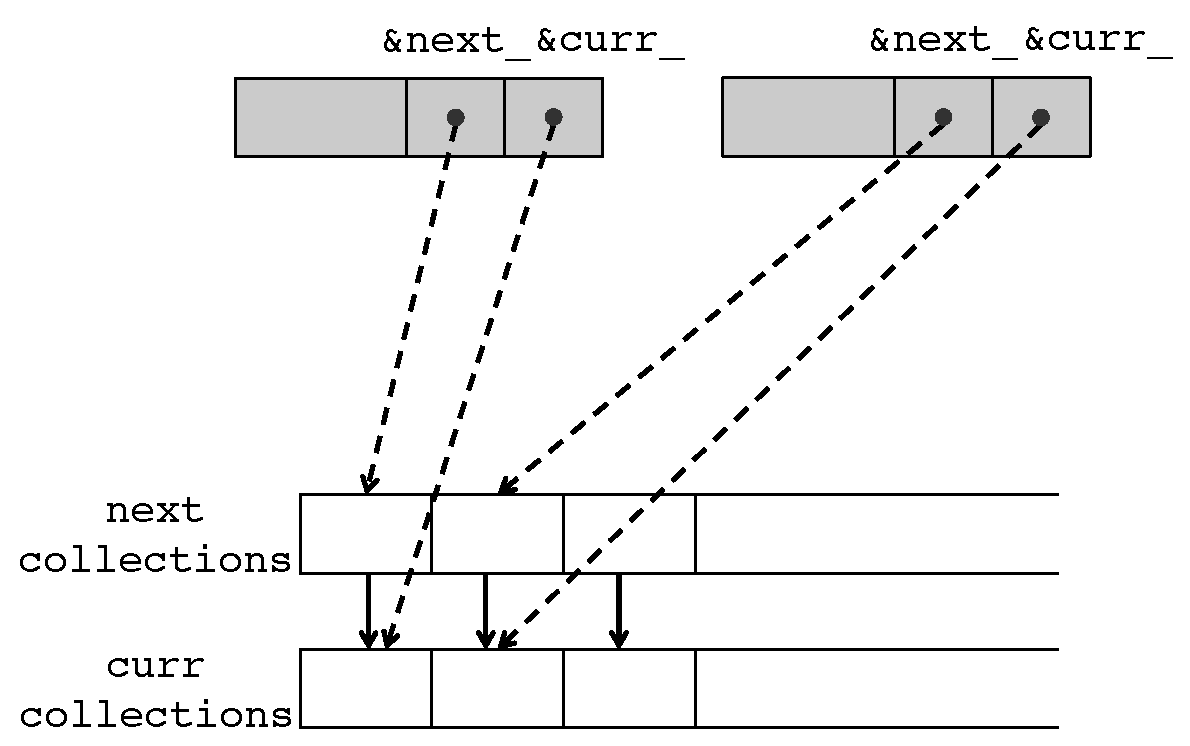
\includegraphics[clip,width=\linewidth-30pt]{registers_mem}
 \caption{値を配列として格納しメモリ配置を工夫した reg クラスのインスタンスの処理の様子}
 \label{fig:mem_copy}
\end{figure}

提案手法について述べる.
\figref{fig:mem_copy} に値を配列として格納しメモリ配置を工夫した reg クラスのインスタンスの処理の様子を示す.
\figref{fig:mem_copy} は提案手法である.
提案手法では全 reg クラスのインスタンスは現在の値と次サイクルの値の実体は持たず,ポインタを保持するように変更している.
reg クラスのインスタンスが灰色に塗られており,左からクラスのメタデータ,\&next\_, \&curr\_ を表している.
\&next\_, \&curr\_ は next\_, curr\_ のポインタである.
下の枠が next\_, curr\_ の値をまとめた配列であり,
ここでは next collections, curr collections と呼ぶ.
実線矢印は代入を表し,点線矢印はポインタの参照先を表す.

ArchHDL の実装では次サイクルに移る前に行われる curr\_ に next\_ の値を代入する処理は
reg クラスのインスタンスが存在するアドレスを調べる必要がある.
しかし値を配列として格納しメモリ配置を工夫すると\figref{fig:mem_copy} に示すように単純な代入となる.
また今まで飛び飛びのアドレスに格納されていた next\_ と curr\_ のメモリ配置がまとまるのでメモリアクセスが連続的に行える.
さらに reg::Update() の関数呼び出しが不要となり,関数呼び出しのオーバーヘッドもなくなる.
これらの理由により高速化が期待できる.

提案手法の実装について述べる.
next collections, curr collections として 2 つの十分大きな \verb/unsigned int/ 型の配列を用意する.
記述された型に応じて,reg クラスのコンストラクタが next\_, curr\_ それぞれの領域を next collections, curr collections に確保する.
確保する領域は参照の高速化のために 4 バイトの倍数とする.
確保された next\_ と curr\_ のアドレスを取得し,インスタンス内の \&next\_, \&curr\_ がそれを保持する.
これまで reg クラスの全インスタンスの reg::Update() メソッドを呼び出していたところを next\_ collections から curr\_ collections の値コピーに変更する.


\if0
\subsection{ダブルバッファリング}

これまでの実装では \ref{ss:implementation} 章で述べたように
reg クラスのインスタンスの次サイクルの値が次サイクルに移る前に reg クラスのインスタンスの現在の値に代入される.
そこで偶数回目の実行と奇数回目の実行で次サイクルの値と現在の値を格納している変数をを入れ替えれば
(ダブルバッファリング)代入が減ることが期待できる.

\begin{figure}[t]
 \begin{center}
  \input{img/reg_curr_next}
 \end{center}
 \caption{reg クラスのインスタンスの変数保持の処理の様子}
 \label{fig:reg_curr_next}
\end{figure}

\begin{figure}[t]
 \begin{center}
  \input{img/double_buffer2}
 \end{center}
 \caption{ダブルバッファリングの処理の様子}
 \label{fig:double_buffer}
\end{figure}

\figref{fig:reg_curr_next} はこれまでの ArchHDL の reg クラスのインスタンスの値の保持のイメージである.
読み込み用と書き込み用の変数をそれぞれ保持している.
読み込み用が現在の値であり,書き込み用が次サイクルの値である,
次サイクルに移る前に書き込み用の値が読み込み用の変数に書き込まれる.

\figref{fig:double_buffer}
はダブルバッファリングのイメージである.
奇数回目のサイクルと偶数回目のサイクルで読み込み用と書き込み用の変数を入れ替える.
これにより奇数回目のサイクルで書き込み用であった変数には値が書き込まれているので次サイクルの偶数回目のサイクルで読み込み用として使用出来る.
これを繰り返すことで,次サイクルに移る前に行われる代入処理を無くせる.

しかし今回の手法では reg クラスのインスタンスへ値の書き込みが行われなかった場合に
reg クラスのインスタンスのその時の書き込み用の値に更新が入らない.
次サイクルではその書き込み用の値がそのまま現在の値として使用されるので古い値が使われてしまう.
そのため単純に入れ替えるだけの実装では誤ったシミュレーションを行なってしまう.

また今回の手法はサイクルの回数で依存関係が発生するので \ref{ss:parallel} 節で述べる並列化ができない.

よってライブラリの実装として導入するのは困難であるが,
reg クラスのインスタンスへ常に書き込みが行われるカウンタ回路で試したところ効果があった(具体的な数字).
常に reg クラスのインスタンスに書き込みが行われるハードウェアシミュレーションを逐次処理で行いたい場合には高い効果が期待できる.

以上の理由から本論文ではダブルバッファリングによる評価は行わない.

\fi

\section{並列化による高速化} \label{ss:parallel}

これまで逐次プログラミングにおける高速化を考えてきたが,本節では並列化による高速化について考える.

\figref{src:class_singleton} の 40 行〜 47 行に示すように
毎サイクル,Module クラスと reg クラスの全インスタンスの Module::Always() メソッドと reg::Update() メソッドが呼び出されている.

\figref{src:class_singleton} の41行〜43行で実行される Module::Always() メソッドはユーザが自由に記述できる.
そのため各 Module クラスのインスタンスで独立に Module::Always() メソッドが実行できる保証はない.
しかしここでは独立に実行できると仮定する.
独立に実行できる条件は今後の研究課題とする.
この場合\figref{src:class_singleton} の41行〜43行に示している Module::Always() メソッドの実行は並列化が可能である.

\figref{src:class_singleton} の 44 行〜 46 行で行われるレジスタの更新は\figref{fig:regs} の実線で表されている.
各インスタンスで独立に行えるので並列化が可能である.

\figref{src:class_singleton} の41行〜47行に示している Module クラスと reg クラスの全インスタンスの Module::Always() メソッドと reg::Update() メソッドの実行は並列化が可能である.
提案手法について述べる.この部分を並列化する.並列化には OpenMP~\cite{openmp} を用いる.

\begin{figure}[t]
 \lstinputlisting[language=c++]{src/exec_openmp.cc}
 \caption{Exec メソッド内の for 文を OpenMP で並列化したプログラム}
 \label{src:exec_openmp}
\end{figure}

\figref{src:exec_openmp} は\figref{src:class_singleton} の 40 行〜 47 行が 8 スレッドで並列化が行われるように OpenMP 指示文を与えたソースコードである.
2 行目は並列化を何スレッドで行うかを与えている.
今回は 8 をスレッド数に指定している.この数字は環境によって変えることができる.
4 行目と 8 行目は for 文の実行を並列化する OpenMP 指示文である.

一般に,並列化を行う場合は各スレッドに対して均等に負荷を与えることが重要である.
OpenMP では for 文の負荷を分散するスケジュール方法として,静的に決定する static や,動的に決定する dynamic など複数の方法が存在する.
一般に,スケジュール方法に dynamic を指定した場合,各スレッドに割り当てられる負荷が均等に近くなるメリットはあるが,オーバーヘッドが大きいデメリットがある.
ArchHDL により記述されたハードウェア記述では各モジュールと各レジスタの負荷が大幅に変わらないのであれば,static を指定した方が効率が良いと考えられる.

他にも OpenMP にはオプションとしてチャンクサイズを指定できる.
スケジュール方法を static にし,チャンクサイズを指定しなければ,チャンクサイズはループの反復数をスレッド数で割った商とほぼ同じ値になる.

今回の評価ではスケジュール方法は static でチャンクサイズは指定しないデフォルトの設定で行う.
